\documentclass[runningheads]{llncs}

\usepackage{dialogue}
\usepackage{tabularx}
\usepackage{float}
\usepackage{amsmath}
\usepackage{subcaption} 
\usepackage[T1]{fontenc}
\usepackage{graphicx}


\begin{document}
%
\title{Comparing RAG and GraphRAG for Page-Level Retrieval Question Answering on Math Textbook}
%
\author{Eason Chen, Chuangji Li, Shizhuo Li, Zimo Xiao, Jionghao Lin, and Kenneth R. Koedinger}
%
\authorrunning{Eason Chen et al.}
%
\institute{Carnegie Mellon University}
%
\maketitle 

\begin{abstract}
Technology-enhanced learning environments often help students retrieve relevant learning content for questions arising during self-paced study.
Large language models (LLMs) have emerged as novel aids for information retrieval during learning. While LLMs are effective for general-purpose question-answering, they typically lack alignment with the domain knowledge of specific course materials such as textbooks and slides. We investigate Retrieval-Augmented Generation (RAG) and GraphRAG, a knowledge graph-enhanced RAG approach, for page-level question answering in an undergraduate mathematics textbook. While RAG has been effective for retrieving discrete, contextually relevant passages, GraphRAG may excel in modeling interconnected concepts and hierarchical knowledge structures. We curate a dataset of 477 question–answer pairs, each tied to a distinct textbook page. We then compare the standard embedding-based RAG methods to GraphRAG for evaluating both retrieval accuracy—whether the correct page is retrieved—and generated answer quality via F1 scores.
Our findings show that embedding-based RAG achieves higher retrieval accuracy and better F1 scores compared to GraphRAG, which tends to retrieve excessive and sometimes irrelevant content due to its entity-based structure. We also explored re-ranking the retrieved pages with LLM and observed mixed results, including performance drop and hallucinations when dealing with larger context windows. Overall, this study highlights both the promises and challenges of page-level retrieval systems in educational contexts, emphasizing the need for more refined retrieval methods to build reliable AI tutoring solutions in providing reference page numbers.
\end{abstract}
\keywords{Retrieval-Augmented Generation, Math, Question Answering, GraphRAG, Page Ranking, Large Language Models} 


\section{Introduction}\label{sec1}

When students learn in technology-based learning environment, they often need to reference or retrieve relevant information in reading excerpts, textbooks, and other structured text content. Artificially intelligent solutions can help students quickly find and reference relevant sources and excerpts related to questions, facts, and other study objectives during this learning process. Increasingly so, these references are generated by large language models (LLMs), which have shown notable expertise in domains such as mathematics and science \cite{brown2020language,openai2024gpt4technicalreport}. However, while these models excel at providing answers, they often lack direct alignment with specific course materials (e.g., textbooks or lecture notes) and struggle to handle specialized domain knowledge, resulting in suboptimal performance \cite{chen2024systematic,moore2022assessing,nguyen2023evaluating}. In the worst case, these models provide incorrect and hallucinated sources to back up claims \cite{ji2023survey}. How can our field move toward more reliable and accurate curation of learning material in personalized learning supported by LLMs?

Retrieval-augmented generation (RAG) has emerged as a promising solution by combining information retrieval mechanisms as context for LLM to generate outputs \cite{wang2024largelanguagemodelseducation,gao2024retrievalaugmentedgenerationlargelanguage,chen2024systematic}. In RAG, a retriever module first identifies potentially relevant documents or pages from a textbook, followed by a generator module that combines the retrieved content with the user’s query to produce an answer. This two-stage pipeline mitigates ``hallucination'' and helps direct the model’s attention to domain-specific information \cite{han2024improving}. A further refinement of RAG is the variant \textit{GraphRAG}\cite{edge2024localglobalgraphrag}, which extends RAG with a knowledge graph to capture entity relationships and provide more comprehensive retrieved content.

In an educational context, it is important that an AI tutor furnishes correct answers and precisely references the textbook pages and content students need to refer to \cite{DAI2024100299,olney_improving_2024}. Ensuring alignment at the page level not only requires the model to retrieve information from and ground its responses in a clearly defined corpus—rather than relying on pre-trained knowledge, but also enables users to easily locate the referenced material in the textbook to review the original context and verify the AI’s response. In particular, when deploying RAG approaches in mathematics education, enhancing retrieval faithfulness by ensuring AI-generated answers are both accurately sourced and effectively address the question can improve learning outcomes~\cite{chiesurin-etal-2023-dangers,levonian2023retrievalaugmentedgenerationimprovemath}. Providing explicit pointers, like page references, might further help students reference for deeper understanding or verify correctness.
% In our paper, we explore how RAG-based pipelines can be adapted for math textbook question answering, focusing on a single \textbf{R}esearch \textbf{Q}uestion (\textbf{RQ}):
In our paper, we explore how RAG-based pipelines can be adapted for math textbook question answering, focusing on the following \textbf{R}esearch \textbf{Q}uestion: \emph{``To what extent can an AI-based retrieval system identify the correct textbook page for a question derived from that specific page?''} 

Specifically, we compare two RAG approaches: a standard embedding-based RAG and a knowledge-graph-based GraphRAG \cite{edge2024localglobalgraphrag} approach that uses graph-structured relationships between mathematical entities. We benchmark these methods on a custom-built dataset of 477 question-answer pairs derived from \emph{An Infinite Descent into Pure Mathematics} \cite{newstead2024infinite}, an undergraduate mathematics textbook. By measuring both retrieval correctness (the ability to locate the appropriate page) and generative quality (the ability to produce the correct answer), our experiments show how different RAG pipelines align large language models more closely with course-specific materials. The findings have direct implications for building reliable AI tutoring systems that not only answer questions but also point learners exactly to where in the textbook they can find references, enabling transparent instruction and mitigating potential hallucinations in LLMs by working in conjunction with existing, verified learning material.


\section{Related Work}

% \subsection{Current Limitation of LLMs in Question Answering}

\subsection{Limitations of LLMs in Question Answering and the Emergence of Retrieval-Augmented Generation (RAG) in Education}

Pre-trained LLMs often struggle to reference specific contextual information. For instance, \cite{moore2022assessing} employed GPT-3 to evaluate student-generated short-answer questions, revealing that the model tends to overestimate question quality and lacks precise alignment with course content. Another study \cite{nguyen2023evaluating} investigated ChatGPT-based feedback with ChatGPT in a digital learning game, finding that the mdoel encountered difficulties with complex number-line problems. These challenges highlight the importance of using augmentation methods like RAG to ensure alignment with educational content.

In response to these limitations, research \cite{chen2024systematic,gao2024retrievalaugmentedgenerationlargelanguage,wang2024largelanguagemodelseducation} indicates that Retrieval-Augmented Generation (RAG) can effectively enhance LLM performance by providing domain-specific context. RAG leverages vector-based embedding retrieval to gather relevant reference documents from an external database, and then feeds the retrieved information to an LLM as input for generation. By grounding model outputs in these context documents, RAG not only helps mitigate hallucination but also boosts factual accuracy. Generally, a RAG pipeline involves two core components: a \emph{retriever}, which indexes and locates relevant snippets or documents (e.g., via semantic embeddings), and a \emph{generator}, which produces the final answer using both the user query and retrieved content. This structure makes RAG particularly appealing for educational settings, where aligning answers with textbook pages, lecture slides, or other course materials can offer significant pedagogical benefits.

Some recent studies have shown the effectiveness of RAG solutions in building LLM-based tutors \cite{han2024improving,mitra2024retllme,feng2024courseassistpedagogicallyappropriateai,henkel2024mathrag,salminen2024cipherbot,lng2025rchat}. Research suggests that these retrieval-based methods not only enhance the accuracy and contextual relevance of automated tutoring but also mitigate hallucinations and other errors in generated responses \cite{han2024improving,zheng2024k12rag}. For instance, RetLLM-E \cite{mitra2024retllme} is a RAG approach designed for university course forums, integrating past Q\&A posts and official course materials to improve LLM-generated responses. Similarly, CourseAssist \cite{feng2024courseassistpedagogicallyappropriateai} is an LLM-based tutor that grounds feedback in lecture slides, notes, and assignments for computer science courses.
% In a K-12 math context, \cite{henkel2024mathrag} found that incorporating RAG with middle-school textbooks improved user satisfaction and reduced off-topic answers. Other work, such as Cipherbot \cite{salminen2024cipherbot}, illustrates how retrieval-based systems can enhance factual correctness and student trust by surfacing explicit source materials for validation.
Nevertheless, certain challenges persist—such as transparency of data retrieval \cite{zheng2024k12rag} and the tendency to retrieve excessively large contexts \cite{lng2025rchat}. Taken together, these systems underscore the promise of RAG in enhancing both the correctness and pedagogical alignment of LLM-based tutoring solutions.


\subsection{GraphRAG}

GraphRAG \cite{edge2024localglobalgraphrag} is a framework introduced by Microsoft Research, which extends the standard Retrieval-Augmented Generation (RAG) paradigm by leveraging structured knowledge graphs to improve document retrieval and response generation ~\cite{chen2020review}. Unlike traditional RAG that indexes unstructured documents using dense embeddings, GraphRAG constructs a network of entities and their relationships extracted from the corpus. This knowledge graph serves as a structured semantic layer, enabling more coherent and focused information retrieval—especially valuable in domains where relationships among concepts (e.g., definitions, theorems) are critical.
The GraphRAG pipeline consists of three main components:

\begin{enumerate}
    \item \textbf{Entity and Relation Extraction:} Using large language models, GraphRAG parses raw textual documents (e.g., academic papers, financial reports, or textbooks) to identify entities (such as concepts, objects, or events) and link them via relations (e.g., ``depends on'', ``is a special case of'').
    
    \item \textbf{Graph Construction and Indexing:} These extracted entities and relationships are used to construct a knowledge graph. Each node is associated with a snippet of source content, allowing GraphRAG to maintain traceability to the original document.

    \item \textbf{Graph-Augmented Retrieval and Generation:} Given a user query, the system identifies relevant nodes and subgraphs, retrieves corresponding source content, and generates a response via an LLM. Importantly, this retrieval is guided by semantic proximity and graph connectivity, allowing GraphRAG to surface conceptually related yet non-contiguous information.
\end{enumerate}

This graph-structured approach is particularly well-suited for complex reasoning tasks and thematic synthesis. For example, when answering a question that requires integrating multiple concepts across a math textbook, GraphRAG can follow graph paths through definitions, theorems, and examples to build a coherent contextual narrative. Research has demonstrated that using GraphRAG in question-answering tasks can significantly enhance model performance \cite{he2024g}, even outperforming traditional RAG approaches \cite{lin2024research}.

Though it often provides richer conceptual links, GraphRAG approach may introduce excessive or irrelevant content retrieval when aligning strictly to textbook pages \cite{guo2024graphrag,zhang2025survey,he2024g}. Specifically, GraphRAG retrieves large neighborhoods of connected entities, which can lead to inclusion of loosely related or off-topic content that dilutes retrieval precision. For example, \cite{guo2024graphrag} observed that GraphRAG sometimes degraded performance by injecting distracting or incorrect context, causing LLMs to generate less accurate answers compared to closed-book settings. \cite{zhang2025survey} further noted that as GraphRAG expands multi-hop graph neighborhoods, the context window becomes increasingly noisy—an issue especially problematic for fine-grained tasks like retrieving specific textbook pages. \cite{he2024g} similarly found that GraphRAG tends to surface overly general entities (e.g., “methodology” or “benchmark”) that are not helpful for narrow-scope question answering, underscoring its mismatch with localized retrieval tasks.

\section{Methods} \label{sec3}
All of our data, code, and evaluation pipeline can be found at our GitHub \url{https://github.com/anonymousStars/ectel25}.
By employing retrieval-augmented generation (RAG) and targeted prompt engineering, our aim is to ensure that large language models (LLMs) produce answers firmly grounded in a specified corpus—such as a textbook—while also directing users to the exact pages pertinent to their queries. This strategy not only streamlines the learning process for students but also enriches traditional classroom instruction by enabling rapid access to textbook-aligned explanations. In this study, we undertake a detailed evaluation of various RAG pipelines, focusing on their ability to retrieve precise textbook pages and generate content-appropriate responses. Specifically, we examine how these RAG approaches influence the quality of LLM-generated tutoring outputs, as well as the extent to which they accurately identify the most relevant pages to answer users’ questions.


\subsection{Data Preparation}

As shown in the Indexing part in Figure \ref{fig:rag_pipeline}, in order to approximate a highly specialized instructional environment, we employed the undergraduate-level mathematics textbook \emph{An Infinite Descent into Pure Mathematics} \cite{newstead2024infinite}, authored by Clive Newstead. This textbook is widely adopted in various undergraduate mathematics courses and, therefore, serves as a relevant and substantial corpus for evaluating our tutoring system. We obtained the textbook in PDF format and converted each page to a LaTeX-based Markdown representation using the OpenAI GPT Vision model \cite{openaiVision} for optical character recognition (OCR) \cite{ghiriti2024exploring}. The resulting corpus was then indexed and stored using both an embedding-based RAG and our GraphRAG pipeline, providing a consistent database for downstream retrieval and evaluation.

% \subsection{RAG Pipelining}
% The pipeline we used are shown in Figure \ref{fig:rag_pipeline} we adapt are both embedding-based RAG and Graph RAG. First, a

\begin{figure*}[ht]
    \centering
    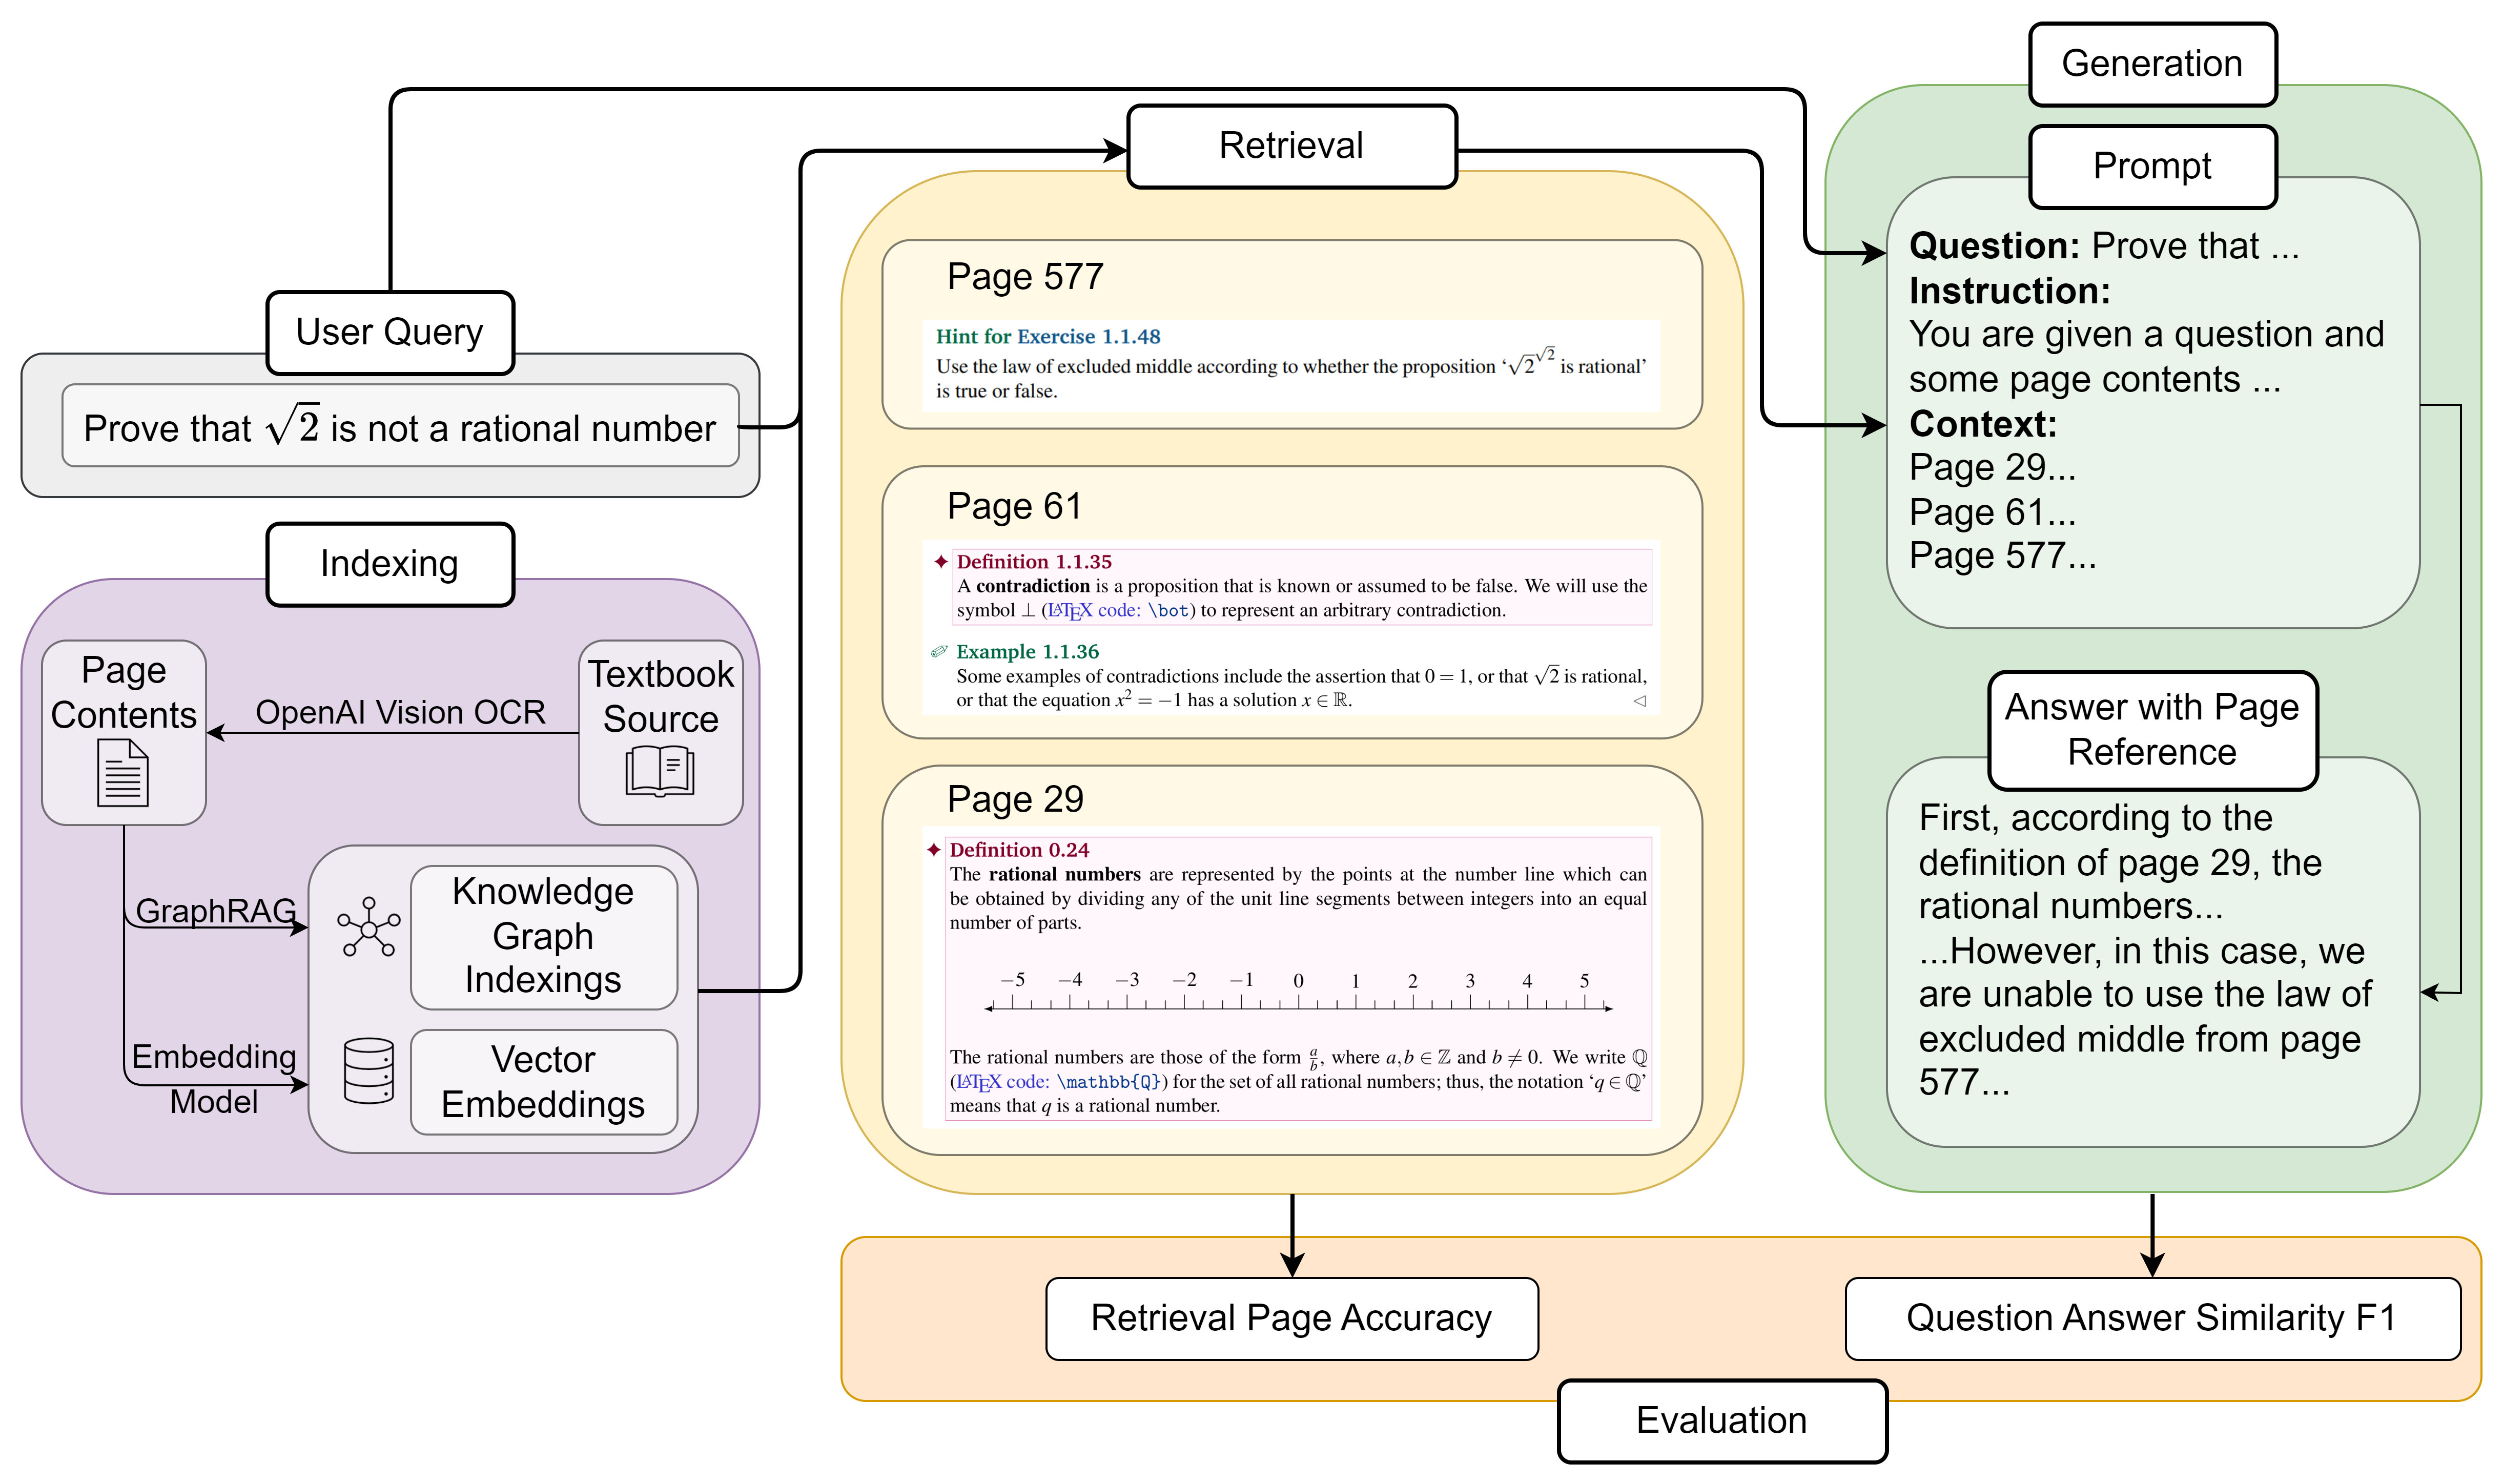
\includegraphics[width=1\linewidth]{images/image.png}
    % \caption{A representative diagram of the RAG process which consists of mainly 3 steps. 1) Indexing. Documents are encoded into vectors by embedding models, or encoded into relational entities by GraphRAG. 2) Retrieval. Retrieve the top-k most relevant pages to the question based on semantic similarity. For GraphRAG, the most relevant entities are retrieved. 3) Generation. Three components are input into LLM: query, prompt, and retrieved pages for final answer. We evaluate the performance of the RAG system with 2 metrics: Firstly, Retrieval Page Accuracy, which measures the probability that the correct page correspond to the question is retrieved. Second, F1. The number of shared words between the output and the truth is the core of the F1 score. Precision is the ratio of the number of shared words to the total number of words in the output, and recall is the ratio of the number of shared words to the total number of words in the truth. And F1 aims to find the balance point between precision and recall.}
    \caption{A representative diagram of our RAG pipeline, which consists of three main steps: (1) \textit{Indexing}, where documents are transformed into vector embeddings or encoded as relational entities with GraphRAG; (2) \textit{Retrieval}, where the system identifies the top-$k$ most relevant pages (or entities) based on semantic similarity; and (3) \textit{Generation}, which uses the query, prompt, and retrieved pages to produce the final answer via an LLM. We measure performance with two metrics: \textit{Retrieval Page Accuracy}, the probability that the correct page is retrieved, and \textit{Question Answer Similarity F1}, computed by comparing shared words in the model output and the ground-truth reference. Precision is the fraction of these shared words relative to the entire output, recall is the fraction of shared words relative to the ground truth, and F1 balances both metrics.}
    \label{fig:rag_pipeline}
\end{figure*}


\subsection{Evaluation Dataset Creation}
Because no existing question-answer pairs are available for this specific textbook, we curated a custom dataset comprising 477 question-answer pairs. The textbook originally contained 628 pages, and we initially created one question per page, totaling 628 questions. Each textbook page yielded exactly one question-answer pair, labeled by its corresponding page number. The process involved prompting a large language model (\texttt{gpt-4o-mini}) with a single page of text at a time, instructing it to generate a mathematically oriented question tied closely to that page’s content, along with a correct, concise answer. These entries were then organized into a JSON structure of the following form: 

\begin{verbatim}
    {
        "page": current page number,
        "title": title of the chapter,
        "content": text content of the page,
        "Question": LLM generated question,
        "Answer": LLM generated answer,
    }
\end{verbatim}

Next, two of the authors, who are highly familiar with the textbook due to relevant coursework, conducted a thorough review and filtering process. We first removed questions generated from the front and back matter, such as headers, index pages, and appendices, reducing the dataset to 528 questions. We then manually reviewed the remaining pages and questions to eliminate any irrelevant content, such as titles, blank pages, and unrelated questions. This process resulted in a final set of 477 question-answer pairs. The final question answer pairs can be found at our GitHub at \url{https://reurl.cc/9D4Yqa}.

\subsection{RAG model selection}


We selected five top-ranking embedding models from the December 2024 Massive Text Embedding Benchmark (MTEB) leaderboard \cite{muennighoff2022mteb,huggingfaceMTEBLeaderboard}. Among these, \texttt{nvidia/nv-embed-v2}, \texttt{voyage-3-large}, and \texttt{intfloat/multilingual-e5-large-instruct} were chosen for their high leaderboard rankings, \texttt{gte-large} is commonly used as a fine-tuning base, and \texttt{OpenAI text-embedding-3-large} was included due to its widespread popularity. Using each of these models for vanilla RAG, we then exhaustively tested retrieval at top-1, top-3, top-5, and top-10, which means how many documents are retrieved and if it includes the target page for accuracy.


\subsection{GraphRAG Adaption}

In our adaptation, we enhanced GraphRAG to expose explicit \texttt{document\_ids} for each knowledge point entity and text unit, ensuring that the model can reference the precise textbook page. Specifically, we modified various GraphRAG components to store and output fields such as \texttt{document\_ids} and \texttt{entity\_ids}, thereby allowing our system to link each retrieved item back to a corresponding page number in \emph{An Infinite Descent into Pure Mathematics}. These modifications introduce additional parameters (e.g., \texttt{include\_document\_ids}) into the context-building functions, enabling more fine-grained control over both the retrieved graph elements and how they are presented to the language model. By adding this information, our GraphRAG not only retrieves a set of relevant entities but also indicates \emph{which page} in the textbook where a student can find the source content. Our modified GraphRAG can be found at GitHub \url{https://reurl.cc/RYzlze}.

\subsection{Evaluation Methodology and Metrics}\label{sec:eval}

As shown in Figure \ref{fig:rag_pipeline}, our evaluation procedure consists of two main components: (1) a machine-based assessment of retrieval accuracy if it contains the target page and (2) a subsequent evaluation of generated answer quality for the question. This two-stage framework reflects the intended educational application of our RAG tutor, specifically within the context of \emph{An Infinite Descent into Pure Mathematics}.

\subsubsection{Retrieval Accuracy} We first assess the \textbf{retrieval accuracy} of our system. For each question in our “one question per page” dataset, we determine whether the model successfully identifies the correct textbook page on which the question is based. In the GraphRAG approach, every retrieved entity is explicitly linked to a particular page, allowing us to verify retrieval quality by comparing the retrieved page indices with the ground-truth page references. We compare GraphRAG performance against embedding-based RAG pipelines that use embedding-based similarity: the corpus is segmented by page, and each page is embedded for search. The top $k$ pages with the highest cosine similarity scores (where $k$ is a tunable hyperparameter) are then retrieved, and the retrieved page indices are matched to the ground-truth page from the dataset. The average retrieval accuracy across $N$ retrievals is computed by averaging number of times correct page $p_i$ exists in the set of retrieved documents $R_i$ for every query $i$ by applying a simple arithmetic mean.

%\[
%\text{Accuracy} \;=\; \frac{1}{N} %\;\sum_{i=1}^{N} \mathbf{1}\,[p_i \;\in\; R_i]
%\]

\subsubsection{Generated Answer Quality}

\begin{table}[h]
    \caption{Target Page Retrieval Accuracy for different models}
    \centering
    \begin{tabular}{lcccc}
        \hline
        Model & Accuracy\\
        \hline
        GraphRAG with o3-mini & 0.914 \\
        GraphRAG with gpt-4o-mini & 0.845 \\
        \hline
        \\
        \hline
        Model &  Top 1 & Top 3 & Top 5 & Top 10 \\ \hline
        gte-large & 0.461 & 0.711 & 0.799 & 0.881 \\ 
        nvidia/nv-embed-v2 & 0.585 & 0.843 & 0.912 & 0.964 \\ 
        voyage-3-large & 0.686 & 0.910 & 0.958 & 0.994\\
        OpenAI text-embedding-3-large & 0.549 & 0.811 & 0.893 & 0.933\\
        intfloat/multilingual-e5-large-instruct & 0.457 & 0.702 & 0.795 & 0.870\\
        \hline
    \end{tabular}
    \label{tab:embedding_result}
\end{table}


\begin{table*}[ht]
    \caption{F1 Score for Answer Generation Performance for different models}
    \centering
    \begin{tabular}{lcccc}
        \hline
        Model & F1 Score\\
        \hline
        gpt-4o-mini & 0.475 \\ 
        GraphRAG with gpt-4o-mini & 0.525 \\
        GraphRAG with o3-mini & 0.524 \\
        \hline
        \\
        \hline
        Model & Top 1 & Top 3 & Top 5 & Top 10 \\ 
        \hline 
        gte-large & 0.526 & 0.533 & 0.550 & 0.552 \\ 
        nvidia/nv-embed-v2 & 0.537 & 0.542 & 0.541 & 0.539 \\ 
        voyage-3-large & 0.523 & 0.543 & 0.544 & 0.547\\
        OpenAI text-embedding-3-large & 0.531 & 0.549 & 0.533 & 0.543\\
        intfloat/multilingual-e5-large-instruct & 0.514 & 0.534 & 0.541 & 0.535\\
        \hline
    \end{tabular}
    \label{tab:answer_f1}
\end{table*}

Next, we evaluate \textbf{generated answer quality} using the \textbf{F1 score}, a standard metric for measuring text similarity in information retrieval and question answering. We used the retrieved information as the context data and let \texttt{gpt-4o-mini} answer the given question, then evaluated the F1 score compared to the original correct answer in the dataset. This F1 score ranges from 0 to 1, where 1 indicates a perfect match between two texts. In our setup, the generated responses are produced by providing the retriever’s results (i.e., the most relevant textbook pages) and the user’s question as context to a generative large language model. In the case of using $R$ to denote the correct answer and $G$ to denote the generated answer. 

To better explain F1 score in this task, we provide an example of calculation. Suppose correct (reference) answer is denoted by $R$ and generative answer is denoted by $G$:

$$\begin{aligned}
    &R = \texttt{"0 is a natural number"}\\
    &G = \texttt{"natural number include 0"}\\
    & |R| = |\{\texttt{0, is, a, natural, number}\}| = 5\\
    & |G| = |\{\texttt{natural, number, include, 0}\}| = 4\\
    & |R \cap G| = |\{\texttt{0, natural, number}\}| = 2\\
\end{aligned}$$

Base on the fact computed above, we compute precision, recall, and F1 score value according to their formulas as follows: 
$$\begin{aligned}
    & \text{precision} = \frac{|R \cap G|}{|R|} = \frac{3}{5};\;\;\;\;\;\;\text{recall} = \frac{|R \cap G|}{|G|} = \frac{3}{4}\\
    & \text{F1} = \frac{2 \times (\textrm{precision} \times \textrm{recall})}{\textrm{precision} + \textrm{recall}} = \frac{2 \times (0.6 \times 0.75)}{0.6 + 0.75} = \frac{0.9}{1.35} \approx 0.667
\end{aligned}$$

We conduct prompt engineering to ensure that the model's answers are both contextually and pedagogically aligned with the textbook material. We then compare the generated answers to the ground-truth answers in our dataset, computing the F1 score for each response. This generative evaluation is performed for GraphRAG, the embedding-based RAG, and a closed-book baseline model, thereby allowing for a direct comparison of their respective accuracies.

\subsection{Re-ranking the output pages}
To ensure an education system can suggest the most relevant reference page number to students, we further tested the performance limit of the retrieval of page numbers by using the re-ranking technique, which orders the retrieved results to improve performance. Specifically, we use \texttt{gpt-4o-mini} to re-rank, providing the model with page contents and their corresponding pages, as well as the question that is potentially based on one of the pages. The LLM then outputs the pages in a Python list format based on the possibility that the question comes from the page, from high to low.

% \subsubsection{Human Evaluation}


\section{Results}\label{sec4}

\begin{table}[b]
    \caption{Retrieval Accuracy change after Page Re-ranking with gpt-4o-mini}
    \centering
    \begin{tabular}{lcccc}
        \hline
        Retrieved Top 5 & Top 1 & Top 3 & Top 5\\
        \hline
        voyage-3-large & 0.686 $\rightarrow$ 0.593 & 0.910 $\rightarrow$ 0.889 & 0.958 $\rightarrow$ 0.958 \\ 
        nvidia/nv-embed-v2 &0.585 $\rightarrow$  0.589&0.843 $\rightarrow$ 0.857 &0.912 $\rightarrow$ 0.912 \\
        OpenAI text-embedding-3-large &0.549 $\rightarrow$  0.585 &0.811 $\rightarrow$ 0.855 &0.893 $\rightarrow$  0.891 \\
        \hline
        \\
        \hline
        Retrieved Top 10 & Top 1 & Top 3 & Top 5 & Top 10\\
        \hline
        voyage-3-large & 0.686 $\rightarrow$ 0.505 & 0.910 $\rightarrow$ 0.841 & 0.958 $\rightarrow$ 0.904 & 0.994 $\rightarrow$ 0.983 \\ 
        nvidia/nv-embed-v2 & 0.585 $\rightarrow$ 0.516 & 0.843 $\rightarrow$ 0.818 & 0.912 $\rightarrow$ 0.870 & 0.964 $\rightarrow$ 0.950 \\
        OpenAI text-embedding-3-large &0.549 $\rightarrow$ 0.491 &0.811 $\rightarrow$ 0.792 &0.893 $\rightarrow$ 0.839 &0.933 $\rightarrow$ 0.919 \\
        \hline
    \end{tabular}
    \label{tab:rerank}
\end{table}
\subsection{Results on Retrieval Accuracy}
% The machine-based auto-evaluation of the testing dataset shows the following result. Both the graph RAG result and the vanilla RAG result are presented. For vanilla RAG, k is set to 1,3,5,10 for exhaustive testing. Five Massive Text Embedding Benchmark (MTEB) top-ranking embedding models at December 2024 \cite{muennighoff2022mteb,huggingfaceMTEBLeaderboard} are selected for vanilla RAG embedding, as shown in Table \ref{tab:embedding_result}. 其中 nvidia/nv-embed-v2, voyage-3-large , intfloat/multilingual-e5-large-instruct  被選擇因為其排名前面，而 gte-large 是許多 Embedding 模型微調的基底，因此也被我們選擇。OpenAI 被選擇則是因為其熱門。


% The machine-based auto-evaluation of the test dataset yields the results presented in Table \ref{tab:embedding_result}, covering both GraphRAG and a baseline (“vanilla”) RAG approach. 


Table \ref{tab:embedding_result} presents the retrieval performance of five leading embedding-based models on our textbook-based question--answer dataset. Notably, \texttt{voyage-3-large} achieves the highest accuracy across all evaluated top-$k$ settings, with a top-1 accuracy of 0.68, improving to 0.91 at top-3, 0.95 at top-5, and reaching 0.99 at top-10. These results indicate that, when allowing up to 10 retrieved pages, \texttt{voyage-3-large} is able to locate the correct page for nearly every question. The second-best performances are achieved by \texttt{nvidia/nv-embed-v2} and \texttt{OpenAI text-embedding-3-large}, with slightly lower but still competitive accuracies. Surprisingly, despite ranking among the top three on the MTEB leaderboard, \texttt{intfloat/multilingual-e5-large-instruct} did not outperform other models from lower ranking. This discrepancy underscores the importance of evaluating embedding models on domain-specific tasks—such as textbook QA—rather than relying solely on general leaderboard standings.

In addition, as shown in Table \ref{tab:embedding_result}, GraphRAG achieved a retrieval accuracy of 0.84 using \texttt{gpt-4o-mini}, and further improved to 0.91 when utilizing \texttt{o3-mini}. Note that since GraphRAG retrieves entire entities instead of ranked pages, we cannot control over the number of pages returned. Consequently, unlike traditional RAG approaches where retrieval results can be explicitly ranked, GraphRAG's accuracy is evaluated based on if the target entity from the page is included in the retrieved data.


% , which are \texttt{thenlper/gte-large}, \texttt{nvidia/nv-embed-v2}, \texttt{voyage-3-large}, \texttt{text-embedding-3-large}, and \texttt{intfloat/multilingual-e5-large-instruct}

\subsection{Result on Generated Answer Quality}

Table \ref{tab:answer_f1} presents the F1 scores for generated answer quality, evaluating how well different models generate responses aligned with the ground-truth answers in the dataset. The evaluation is based on the F1 score, measuring the similarity between the generated content and the correct answer. \texttt{gpt-4o-mini} serves as the foundational language model for generating responses.

The results indicate that incorporating RAG as contextual input consistently improves generative performance compared to the baseline model, which directly generates answers without retrieval, achieving an F1 score of 0.475. Among the single-document retrieval approaches, \texttt{nvidia/nv-embed-v2} surprisingly achieves the best performance, outperforming \texttt{voyage-3-large}, which originally had the highest retrieval accuracy but ranks only third in F1.

For multi-document retrieval, the performance varies based on the number of retrieved documents, with F1 scores ranging between 0.53 and 0.55. Interestingly, while increasing the number of retrieved documents enhances the probability of including the correct reference page, it does not always translate to a better alignment with the target answer. For example, when retrieving three documents, \texttt{nvidia/nv-embed-v2} achieves an F1 score of 0.542, but when increasing to five documents, the score slightly drops to 0.541.

Surprisingly, GraphRAG demonstrates lower generative performance compared to other models, with an F1 score around 0.52. This suggests that while GraphRAG may enhance retrieval by leveraging structured entity relationships, its impact on answer generation is not necessarily superior to traditional embedding-based RAG approaches.


\subsection{Results on Re-ranking}

As shown in Table \ref{tab:rerank}, re-ranking with \texttt{gpt-4o-mini} does not consistently improve retrieval performance, especially in top-1 accuracy. For instance, when using \texttt{voyage-3-large} and re-ranking the top five retrieved pages, the top-1 accuracy drops from 0.686 to 0.593, and further declines to 0.505 when re-ranking the top ten. Nevertheless, some models do improve by re-ranking: for example, \texttt{OpenAI/text-embedding-3-large} improves from 0.549 to 0.585 after re-ranking the top 5. However, its performance in the top 10 also deteriorates from 0.549 to 0.491 after re-ranking. These outcomes suggest that while re-ranking with an LLM may be beneficial, it does not necessarily yield better results when large numbers of documents are involved.

Moreover, we observed instances of hallucination in certain re-ranking scenarios—specifically, when re-ranking the top ten candidates for \texttt{voyage-3-large} and even the top five for \texttt{OpenAI/text-embedding-3-large}. In these cases, the model generated incorrect page numbers or references that do not actually exist, resulting in a slight performance drop compared to the original ranking.


\section{Discussion and Future Works}\label{sec5}


\subsection{The effectiveness using RAG for math QA}

Our results indicate that incorporating RAG leads to more contextually aligned answers compared to baseline using \texttt{gpt-4o-mini}. All RAG approaches yield higher F1 scores. This finding suggests that RAG-based methods can effectively enhance the quality of question responses for mathematics textbook content.

% \subsection{Retrieve the source page by question} \label{sec:page_retrieval}
\subsection{Locating the Correct Page with RAG} \label{sec:page_retrieval}


Despite the noteworthy progress made in RAG, achieving perfect page-level retrieval remains a formidable challenge. In our experiments, the \texttt{voyage-3-large} model successfully located the correct page for a given query 68.6\% of the time, which is significantly better than randomly picking (0.16\%). However, from a practical perspective, a top-1 accuracy below 70\% may not be sufficiently reliable to deploy, especially in settings where students rely on suggested page references.

On the other hand, it is worth re-framing the question so that the absence of the designated ``source'' page in the retrieval set does not invariably count as a failure. In some cases, the RAG system may have identified alternative pages that are more relevant or contain more comprehensive explanations for the question at hand. Thus, one could argue that RAG systems should be evaluated primarily on their ability to retrieve \emph{relevant content} rather than strictly adhering to a particular ``ground-truth'' page label. Future work involving more qualitative assessments of retrieved content and real-world classroom testing will be essential for evaluating the reliability of this approach, particularly when considering deployment in production-level educational environments.


\subsection{RAG vs.\ GraphRAG} \label{subsec:rag_vs_graphrag}

Although GraphRAG presents a promising strategy by leveraging knowledge graphs to retrieve conceptually linked entities, our findings indicate that the standard embedding-based RAG approaches currently outperform GraphRAG in our task: the former yields higher retrieval accuracy (in the Top 5 and above) and a higher F1 score in generated answers. There are two potential reasons that can explain this result:

\noindent{\textbf{1. GraphRAG retrieved too many noises}}
First, while knowledge graphs facilitate the retrieval of relevant entities, they offer limited control over both the number and granularity of these entities. As a result, we observed extraneous pages beyond the one originally associated with a given query may be included, resulting in higher retrieval accuracy but lower F1 scores. This finding is aligned with some previous research \cite{he2024g,zhang2025survey,guo2024graphrag}.

To be specific, our evaluations reveal that GraphRAG retrieves, on average, 46,949 tokens per question as context information. In contrast, the vanilla embedding-based RAG approach using \texttt{voyage-3-large} with top-5 retrieval only retrieves 3,743 tokens on average. The number decreases further for the top 3 (2,339 tokens) and top 1 (899 tokens). These results demonstrate that, compared to GraphRAG, conventional RAG methods can greatly reduce the context window and computational overhead.


\noindent{\textbf{2. GraphRAG retrieved structure is different than page}}
The page-level structure of the textbook—and the generation of questions tied specifically to single pages—does not align smoothly with GraphRAG's entity-based representation. The resulting mismatch between the textbook's linear format and the more fragmented graph-based retrieval may reduce the F1 scores, as the generative model is forced to process unwieldy or redundant contexts \cite{guo2024graphrag,zhang2025survey}. Moreover, extending the context window to accommodate these extra documents can impair the quality of the model's final output, mirroring the diminished performance we observed when retrieving more pages in a standard RAG setting.

Overall, these observations suggest that while GraphRAG introduces promising graph-based mechanisms that can capture local and global relationships among mathematical concepts, it does not yet confer a clear advantage over simpler RAG pipelines in a page-specific retrieval scenario. Future work should investigate methods to adapt GraphRAG's knowledge point structure to align with textbook pages (e.g., by imposing a page-level partition on the underlying graph) and to customize entity selection heuristics (e.g., stricter thresholds), thereby reducing both retrieval noise and excessive context length.

\subsection{The effectiveness of re-ranking}

Our findings reveal that using an LLM to re-rank retrieved page content yields mixed results. While some instances, especially for re-ranking on fewer documents, show improved scores, we observe more frequent score declines and even hallucinations, particularly when dealing with the top-10 scenario, which has a larger context window. This suggests that relying on LLM-based re-ranking is not necessarily effective. Future work should focus on improving LLM performance in document re-ranking (e.g. additional prompt engineering or fine-tuning) to further improve the page locating performance, which is essential for delivering more reliable and accurate content recommendations in educational contexts.


\subsection{Extending the Approach Beyond Page-Level Retrieval}
Beyond pinpointing a textbook page, our approach has broader potential for educational materials across multiple formats—such as mapping questions to specific lecture slides, identifying relevant sections in research papers, or even matching question prompts to timestamps in instructional videos. While traditional indexing methods (e.g., keyword-based or topic-based indexes) often suffice for relatively straightforward lookups, these methods can falter when more personalized or context-rich responses are needed. In contrast, an LLM-based retrieval-augmented generation (RAG) system not only locates relevant sources but also tailors explanations, mitigates ambiguity, and strengthens credibility by grounding the answer in retrieved text. Our experiments suggest that although current retrieval accuracy shows promise, achieving truly fine-grained alignment with the correct page—or comparable unit of reference—remains challenging. 


\subsection{Open-Sourced Dataset and Benchmark Evaluation Code}

To facilitate further research, we have open-sourced our dataset and code at \url{https://github.com/anonymousStars/ectel25}. We believe there is significant potential to develop additional benchmarks and dataset that assess how effectively retrieval systems can locate specific slides, paper sections, or video segments.



\subsection{Limitations}
In this work, due to limited resources, the content was generated with assistance from large language models (LLMs) and evaluated by humans. However, future efforts can build upon the same dataset structure and benchmark code to construct similar evaluation sets using human-authored content. By systematically comparing traditional indexing approaches with more advanced LLMs and LLM-powered pipelines, the research community can gain deeper insights into the trade-offs between simplicity and personalized, source-grounded feedback—ultimately advancing the development of more robust and adaptive tools.


\section{Conclusion}
We investigated the use of Retrieval-Augmented Generation (RAG) and GraphRAG for mathematics textbook question answering, focusing on whether these methods can identify and reference the correct textbook page at a fine-grained level. Our experiments on a custom dataset of 477 question–answer pairs derived from \emph{An Infinite Descent into Pure Mathematics} indicate that embedding-based RAG approaches generally outperform GraphRAG in page-level retrieval, yielding higher accuracy in retrieval and F1 scores in generative answers. While GraphRAG effectively captures conceptual relationships via knowledge graphs, it tends to retrieve excessive content, leading to large context windows that lower generation quality. Additionally, re-ranking retrieved pages by an LLM showed mixed benefits and introduced risks of hallucination under larger context sizes. Overall, these findings underscore the importance of careful design choices—such as page-based chunking and controlled context lengths—when building AI tutors that not only provide accurate answers but also pinpoint the textbook pages to back up claims. Future work may explore more sophisticated techniques to adapt GraphRAG for structured textbooks and broaden the evaluation to larger models and multiple textbooks toward scalable AI-driven educational tools.




%%
%% Print the bibliography
%%
\bibliographystyle{splncs04}
\bibliography{main}

%%
%% If your work has an appendix, this is the place to put it.
%\appendix

%\section{Research Methods}

\end{document}
\endinput
%%
%% End of file `sample-sigconf-biblatex.tex'.
